% latex table generated in R 3.6.3 by xtable 1.8-4 package
% Thu Jan 18 11:49:34 2024
\begin{table}[ht]
\centering
\begin{tabular}{rlrrr}
  \hline
 & OTU & MeanRA & MedianRA & SE \\ 
  \hline
440085 & Methylorubrum extorquens & 0.00006755 & 0.00006182 & 0.00000904 \\ 
  1549855 & Haematospirillum jordania & 0.00003323 & 0.00003227 & 0.00000259 \\ 
  2018065 & Roseomonas sp. FDAARGOS\_36 & 0.00005964 & 0.00005913 & 0.00000374 \\ 
  1296990 & Komagataeibacter xylinus & 0.00005284 & 0.00005642 & 0.00000310 \\ 
  33995 & Komagataeibacter europaeu & 0.00003947 & 0.00003882 & 0.00000367 \\ 
  314260 & Parvularcula bermudensis & 0.00007076 & 0.00007245 & 0.00000326 \\ 
  2811789 & Burkholderia sp. MS38 & 0.00006783 & 0.00007479 & 0.00000491 \\ 
  1795043 & Burkholderia sp. PAMC 2656 & 0.00005509 & 0.00005733 & 0.00000421 \\ 
  2811788 & Burkholderia sp. MS45 & 0.00006243 & 0.00006406 & 0.00000421 \\ 
  1636423 & Burkholderia sp. MSMB158 & 0.00001515 & 0.00001336 & 0.00000299 \\ 
  2584944 & Sutterella faecali & 0.00007985 & 0.00008153 & 0.00000552 \\ 
  557598 & Laribacter hongkongensis & 0.00003195 & 0.00002929 & 0.00000200 \\ 
  2726956 & Pseudomonas sp. MSPm & 0.00007215 & 0.00004760 & 0.00001621 \\ 
  2749999 & Pseudomonas sp. RtIB02 & 0.00005491 & 0.00005389 & 0.00000679 \\ 
  2049589 & Pseudomonas sp. HLS- & 0.00005430 & 0.00004614 & 0.00000900 \\ 
  2774873 & Pseudomonas sp. ADP & 0.00005263 & 0.00004501 & 0.00000868 \\ 
  1649877 & Pseudomonas sp. CCOS 19 & 0.00004227 & 0.00003933 & 0.00000473 \\ 
  2025658 & Pseudomonas sp. NS1(2017 & 0.00002542 & 0.00002226 & 0.00000391 \\ 
  198620 & Pseudomonas koreensi & 0.00006890 & 0.00007122 & 0.00000587 \\ 
  702115 & Pseudomonas arsenicoxydan & 0.00006397 & 0.00005599 & 0.00000574 \\ 
  1691904 & Pseudomonas sedimini & 0.00006111 & 0.00003881 & 0.00001474 \\ 
  86265 & Pseudomonas thivervalensi & 0.00005030 & 0.00004030 & 0.00000612 \\ 
  1853130 & Pseudomonas silesiensi & 0.00004777 & 0.00004883 & 0.00000468 \\ 
  46677 & Pseudomonas agaric & 0.00005192 & 0.00004550 & 0.00000601 \\ 
  1134687 & Klebsiella michiganensi & 0.00003658 & 0.00004575 & 0.00000603 \\ 
  1646377 & Rouxiella badensi & 0.00003420 & 0.00003593 & 0.00000242 \\ 
  1484158 & Pantoea sp. PSNIH & 0.00002673 & 0.00002547 & 0.00000194 \\ 
  472759 & Nitrosococcus halophilus & 0.00002257 & 0.00002061 & 0.00000224 \\ 
  2686360 & Cobetia sp. L2A & 0.00004663 & 0.00004837 & 0.00000204 \\ 
  2738883 & Candidatus Reidiella endopervernicos & 0.00004762 & 0.00004830 & 0.00000354 \\ 
  67258 & Streptomyces cavourensi & 0.00006802 & 0.00007128 & 0.00000516 \\ 
  75293 & Streptomyces autolyticu & 0.00005443 & 0.00004622 & 0.00001045 \\ 
  145458 & Rathayibacter toxicu & 0.00003738 & 0.00003751 & 0.00000272 \\ 
  37929 & Glutamicibacter nicotiana & 0.00003259 & 0.00002934 & 0.00000260 \\ 
  85693 & Mycolicibacterium monacens & 0.00004666 & 0.00005015 & 0.00000382 \\ 
  191292 & Rhodococcus aetherivoran & 0.00002537 & 0.00002447 & 0.00000284 \\ 
  152794 & Corynebacterium efficien & 0.00005186 & 0.00004623 & 0.00000389 \\ 
  39791 & Corynebacterium glucuronolyticu & 0.00004739 & 0.00004871 & 0.00000333 \\ 
  38288 & Corynebacterium genitaliu & 0.00003945 & 0.00004418 & 0.00000263 \\ 
  181487 & Schaalia cardiffensi & 0.00003525 & 0.00003417 & 0.00000204 \\ 
  2609299 & Actinobaculum & 0.00003736 & 0.00003635 & 0.00000306 \\ 
  2636013 & Adlercreutzia & 0.00003636 & 0.00003639 & 0.00000239 \\ 
  2490858 & Staphylospora marin & 0.00006211 & 0.00006479 & 0.00000552 \\ 
  2610894 & Flintibacter & 0.00004137 & 0.00003964 & 0.00000333 \\ 
  271 & Thermus aquaticu & 0.00007097 & 0.00007814 & 0.00000643 \\ 
  2528007 & Polystyrenella long & 0.00005662 & 0.00005123 & 0.00000405 \\ 
  1441386 & Athalassotoga saccharophil & 0.00000714 & 0.00000656 & 0.00000158 \\ 
  430914 & Halorhabdus tiamate & 0.00003846 & 0.00003784 & 0.00000297 \\ 
  62320 & Haloterrigena turkmenic & 0.00007049 & 0.00007346 & 0.00000486 \\ 
  370324 & Natrinema longu & 0.00004589 & 0.00004905 & 0.00000359 \\ 
  1175445 & Methanocella arvoryza & 0.00002872 & 0.00003059 & 0.00000219 \\ 
  1293037 & Thermococcus celer & 0.00001145 & 0.00001047 & 0.00000107 \\ 
  1470066 & Nitrosopumilus cobalaminigene & 0.00000748 & 0.00000680 & 0.00000222 \\ 
  1353260 & Candidatus Nitrosocosmicus oleophilu & 0.00007434 & 0.00008687 & 0.00001041 \\ 
  2259672 & Candidatus Nitrosotenuis sp. DW & 0.00000799 & 0.00000754 & 0.00000231 \\ 
   \hline
\end{tabular}
\caption{Keystone OTUs of } 
\end{table}
\begin{figure}
\centering
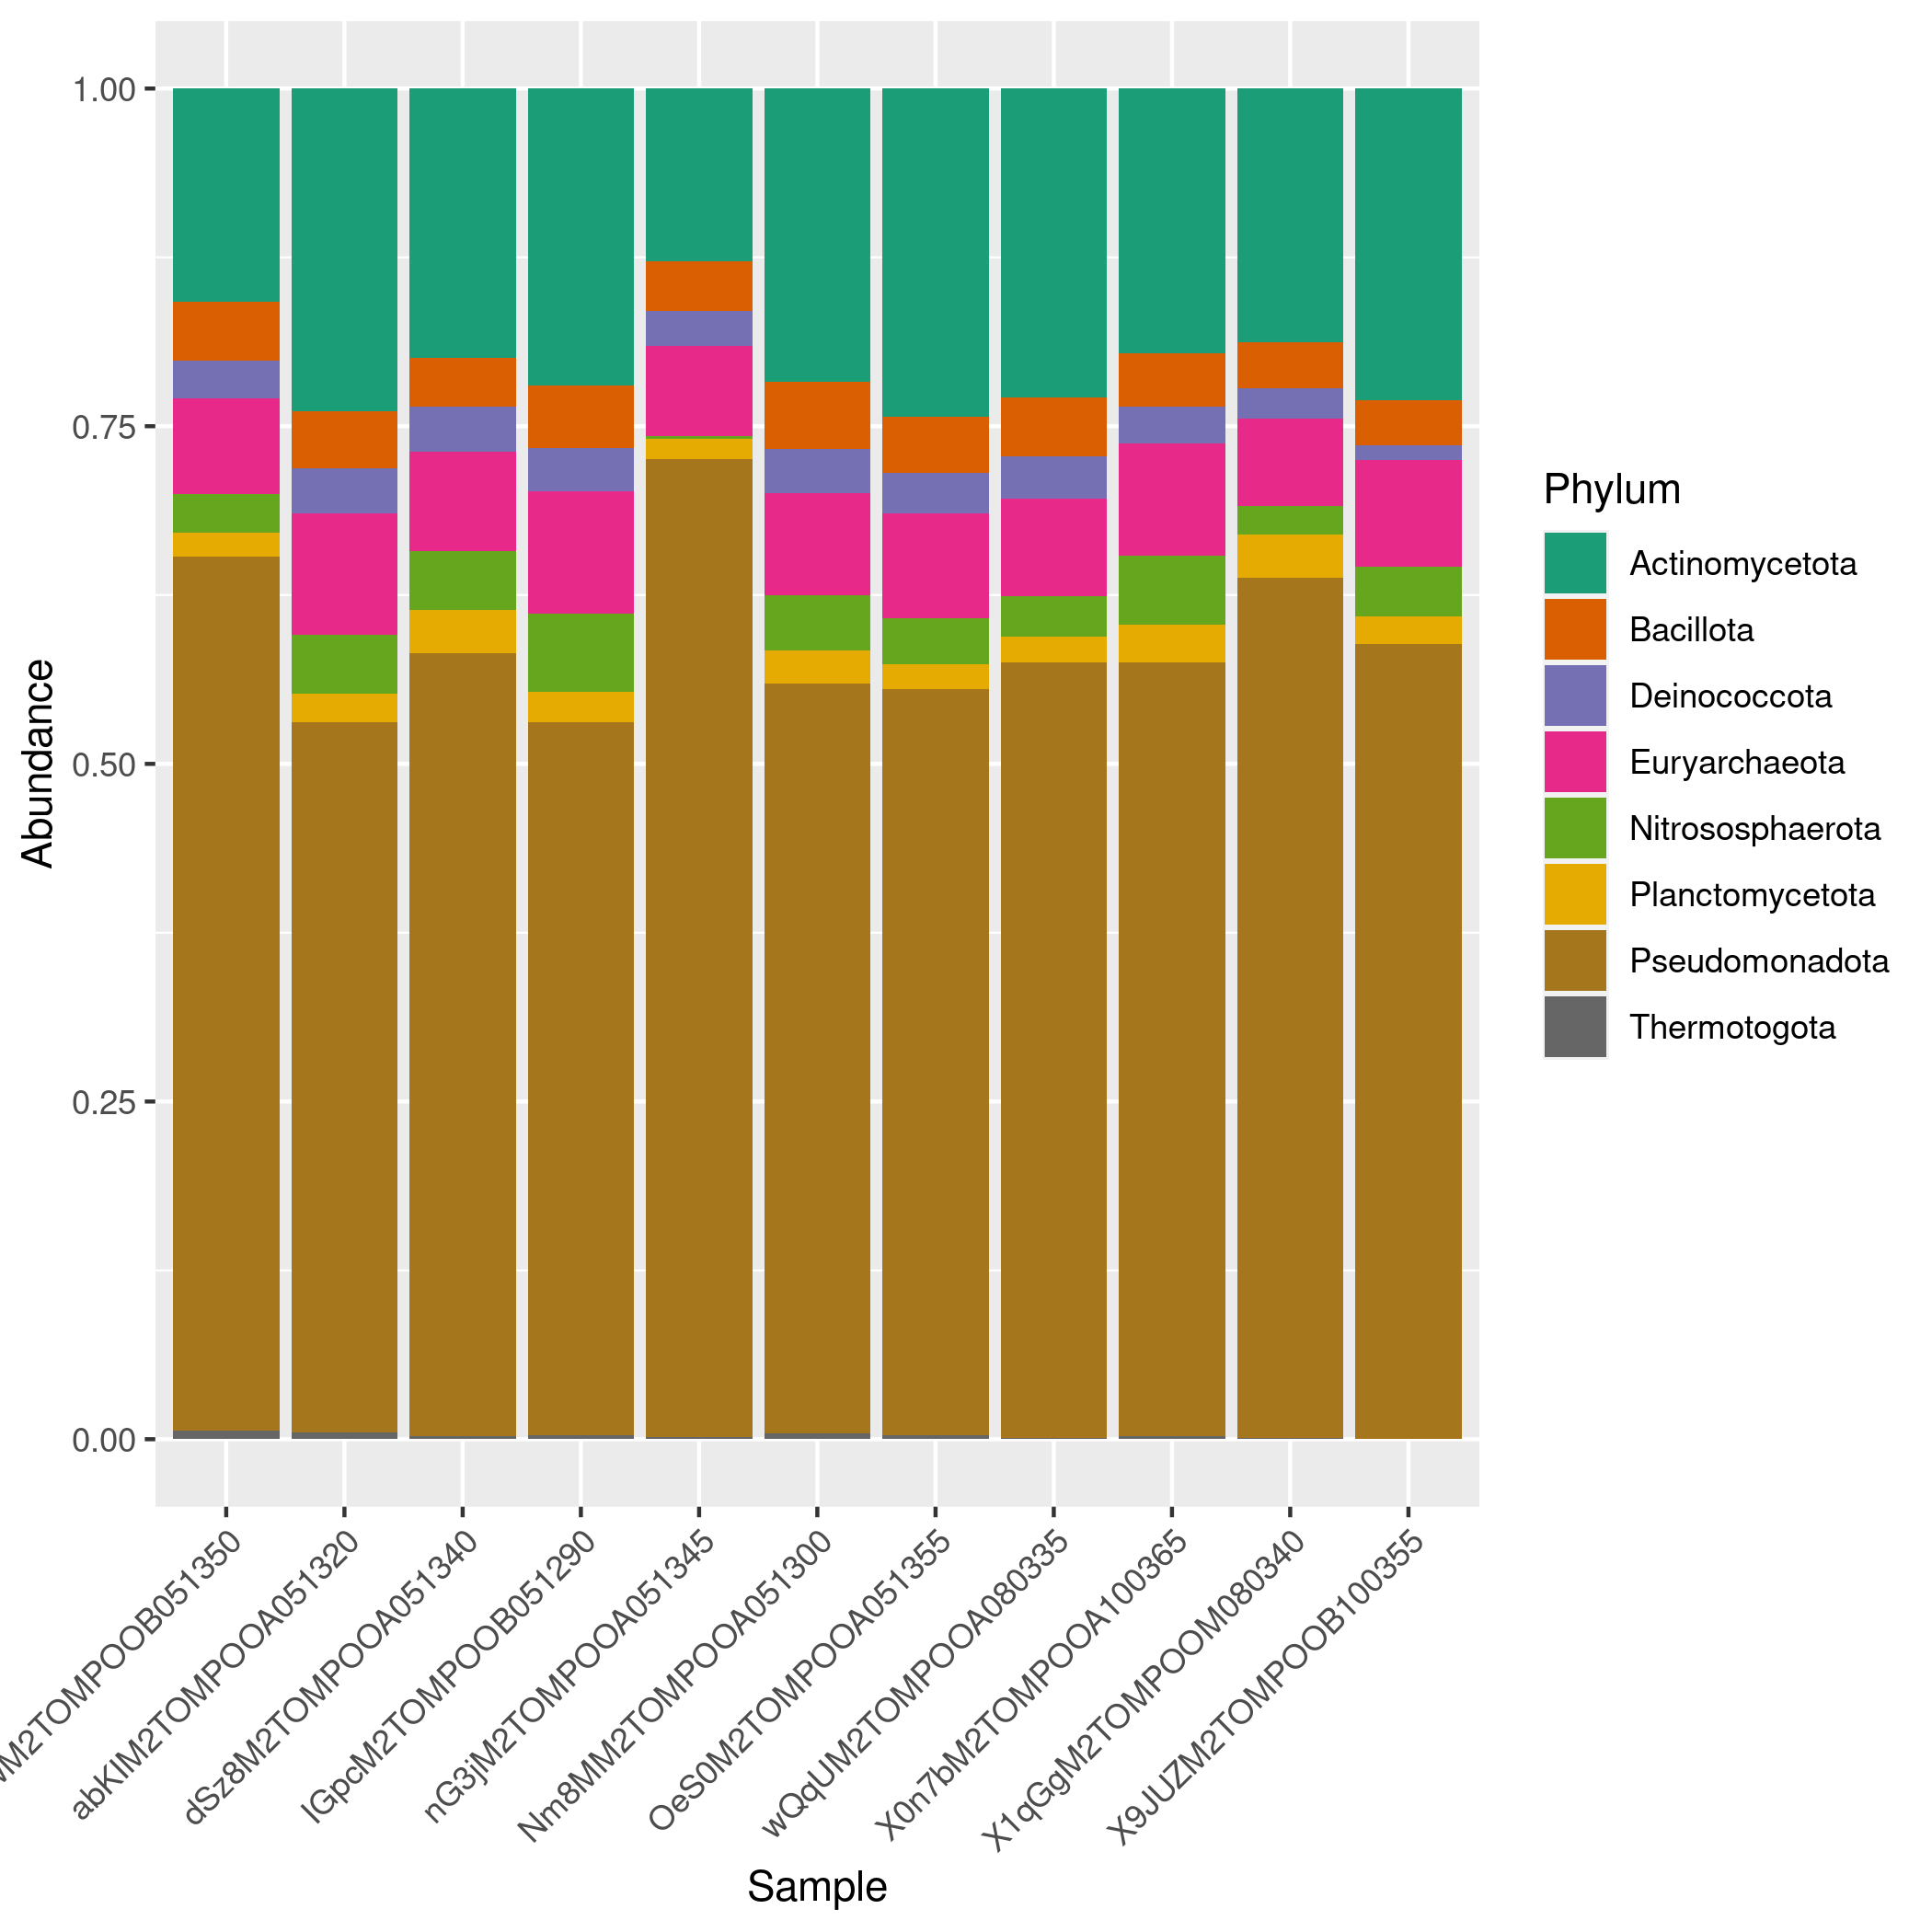
\includegraphics[scale = 0.8]{tomate_aleatorio1_9.csv_relative_abundance_Phylum.png}
\caption{Relative abundance by phyla of keystone OTUs }
\label{fig:tomate_aleatorio1_9.csv_phyla}
\end{figure}
\begin{figure}
\centering
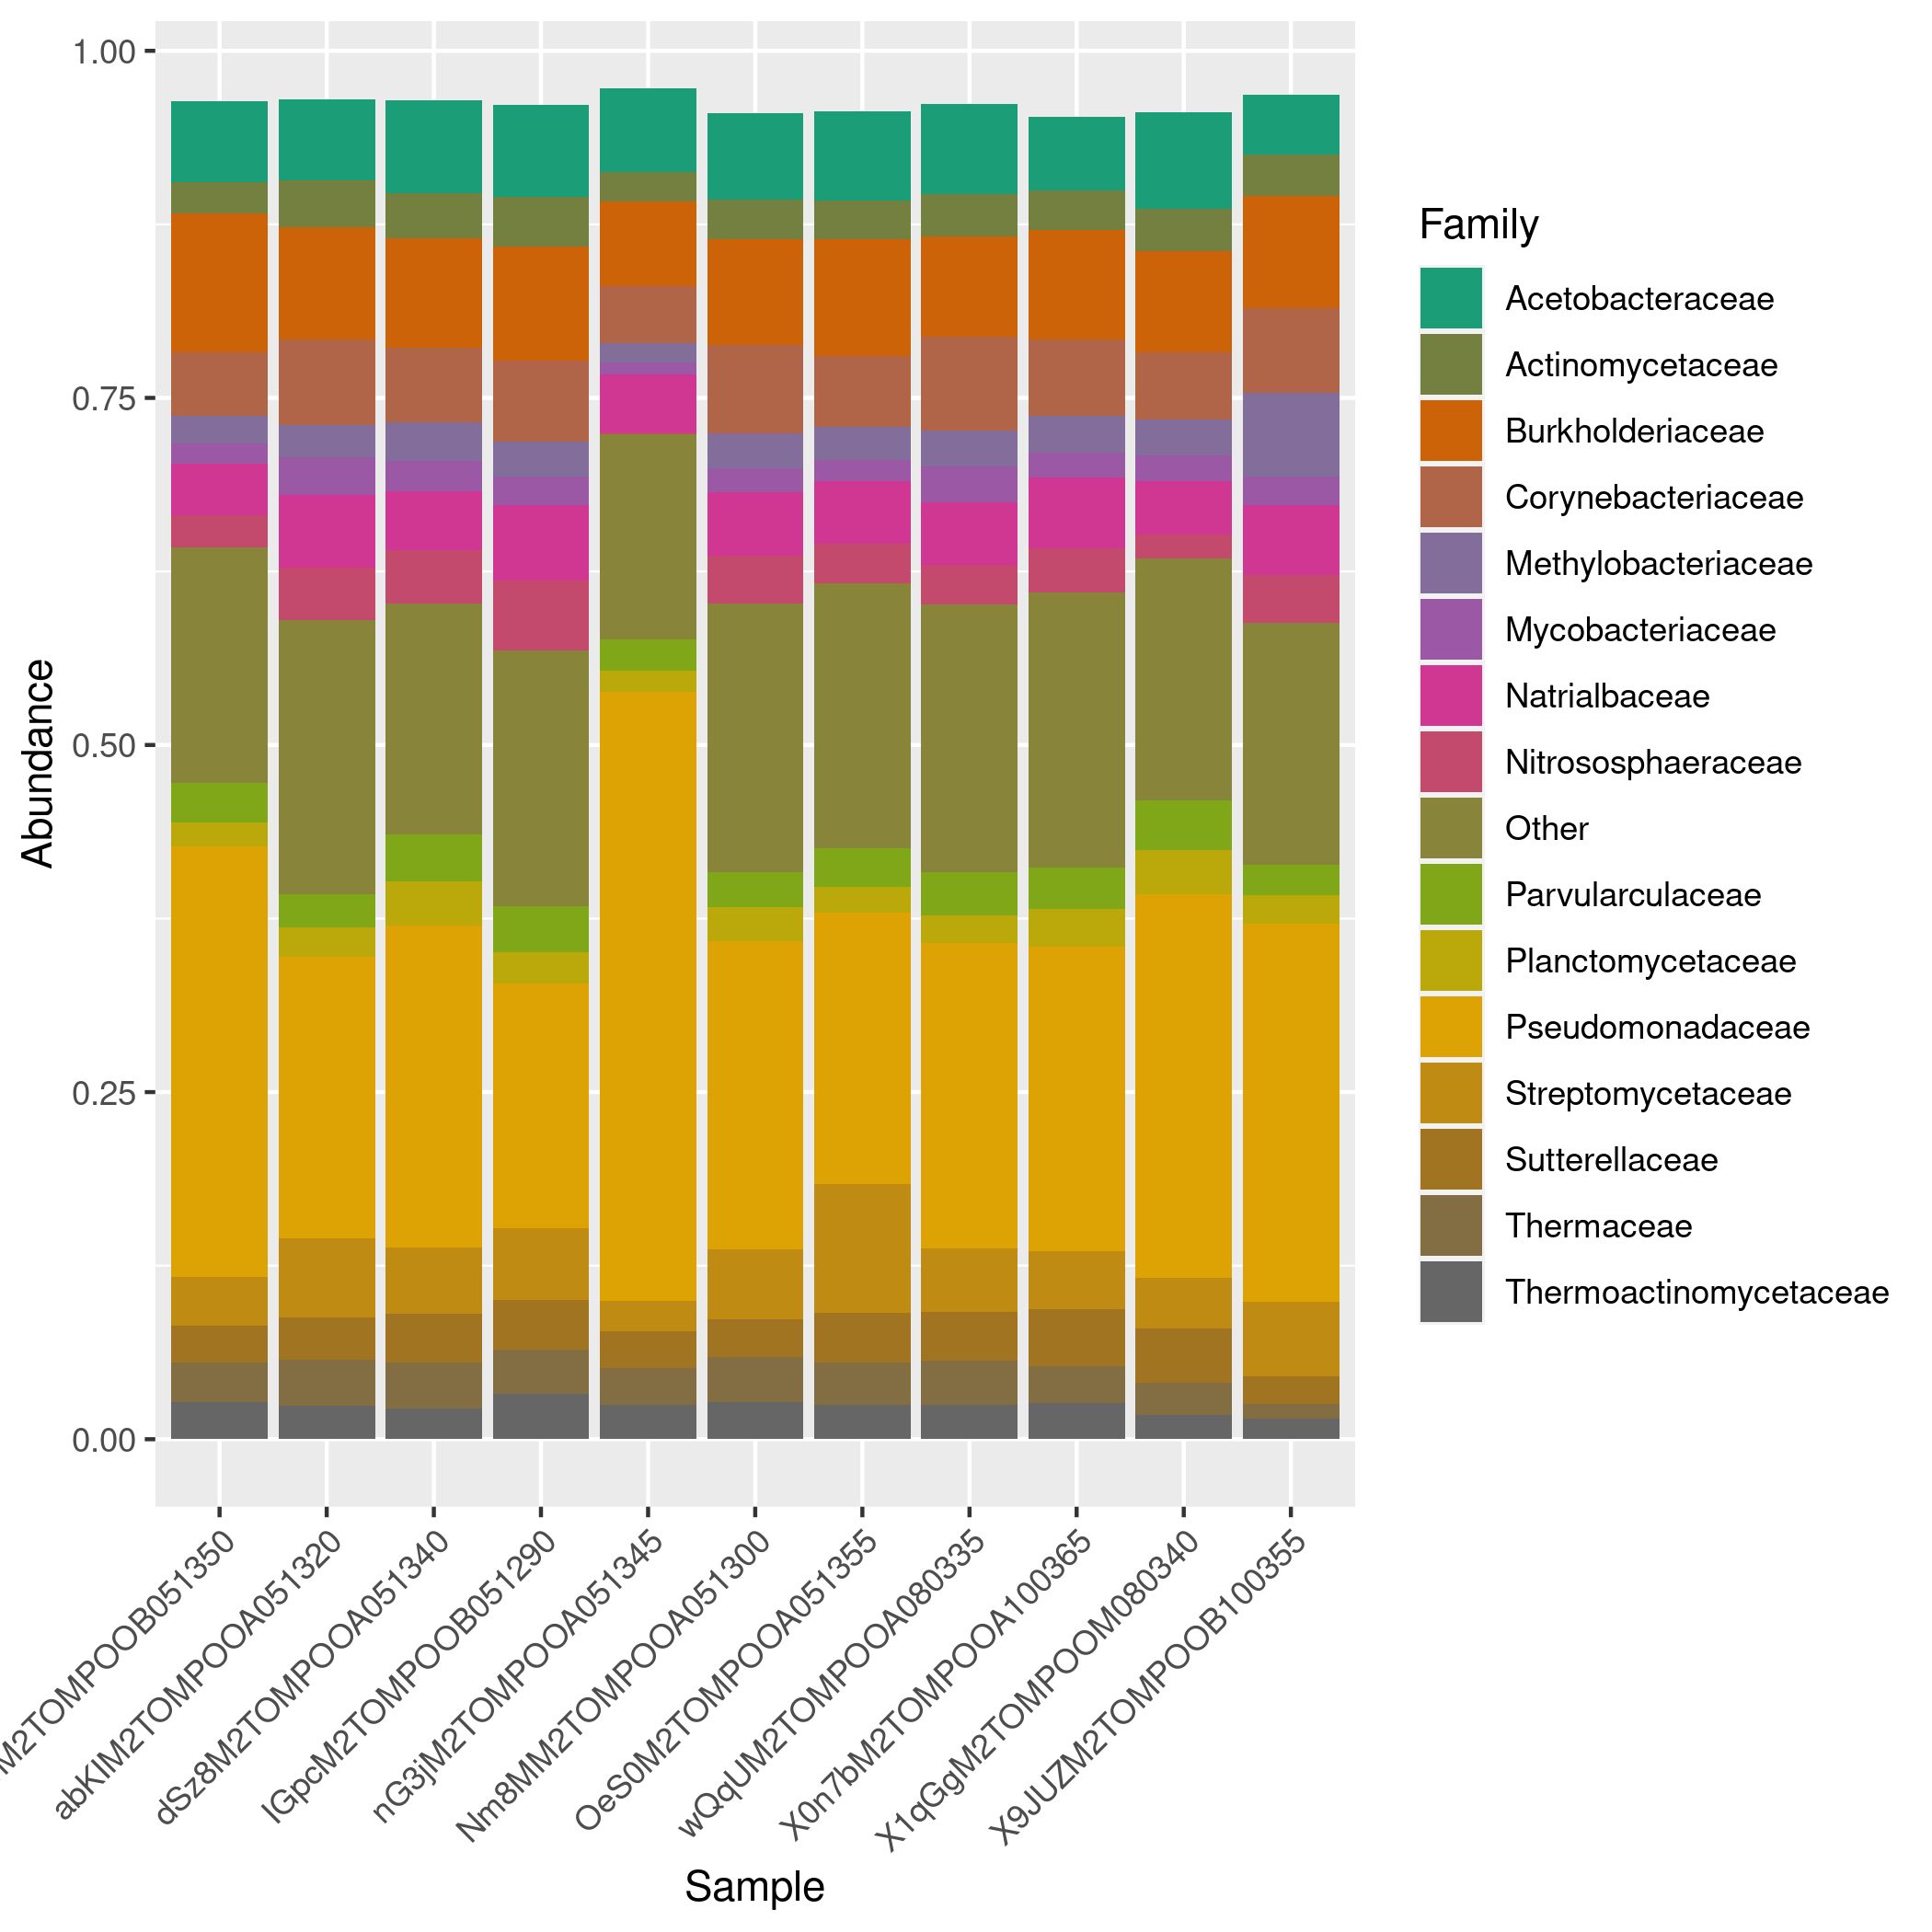
\includegraphics[scale = 0.8]{tomate_aleatorio1_9.csv_relative_abundance_Family.png}
\caption{Relative abundance by families of keystone OTUs }
\label{fig:tomate_aleatorio1_9.csv_family}
\end{figure}
\begin{figure}
\centering
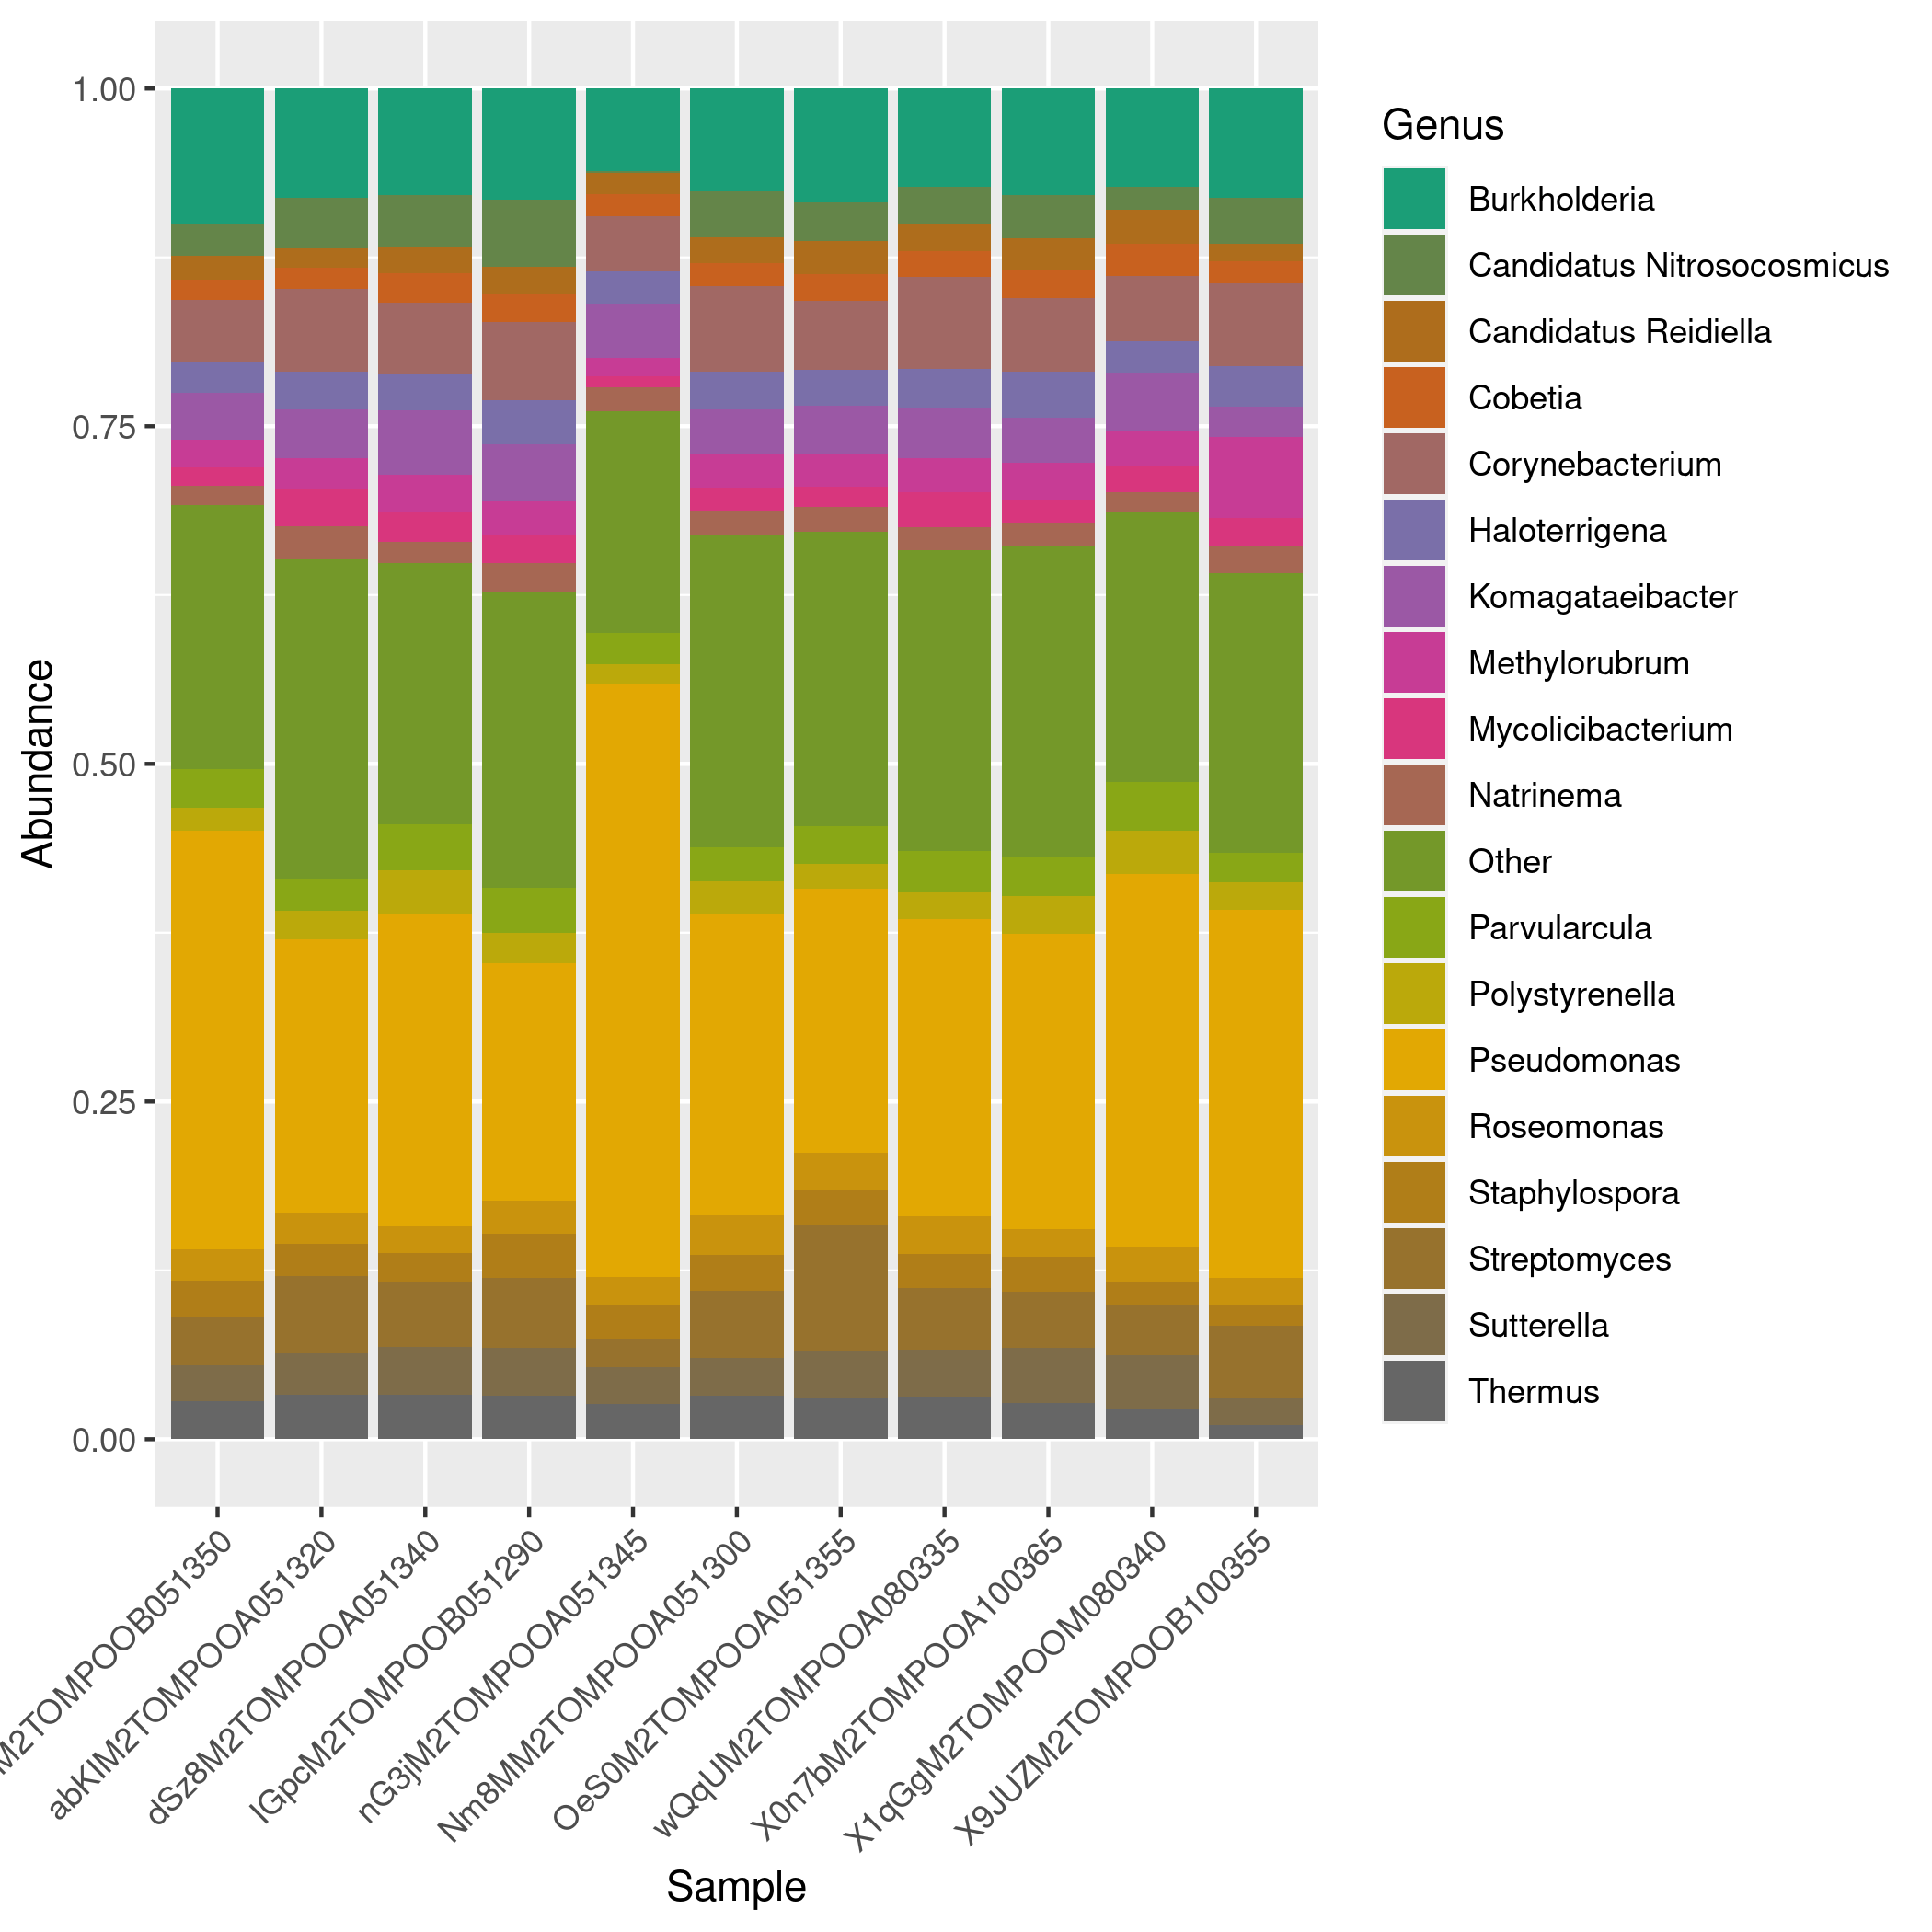
\includegraphics[scale = 0.8]{tomate_aleatorio1_9.csv_relative_abundance_Genus.png}
\caption{Relative abundance by genera of keystone OTUs }
\label{fig:tomate_aleatorio1_9.csv_genus}
\end{figure}
\begin{figure}
   \centering
   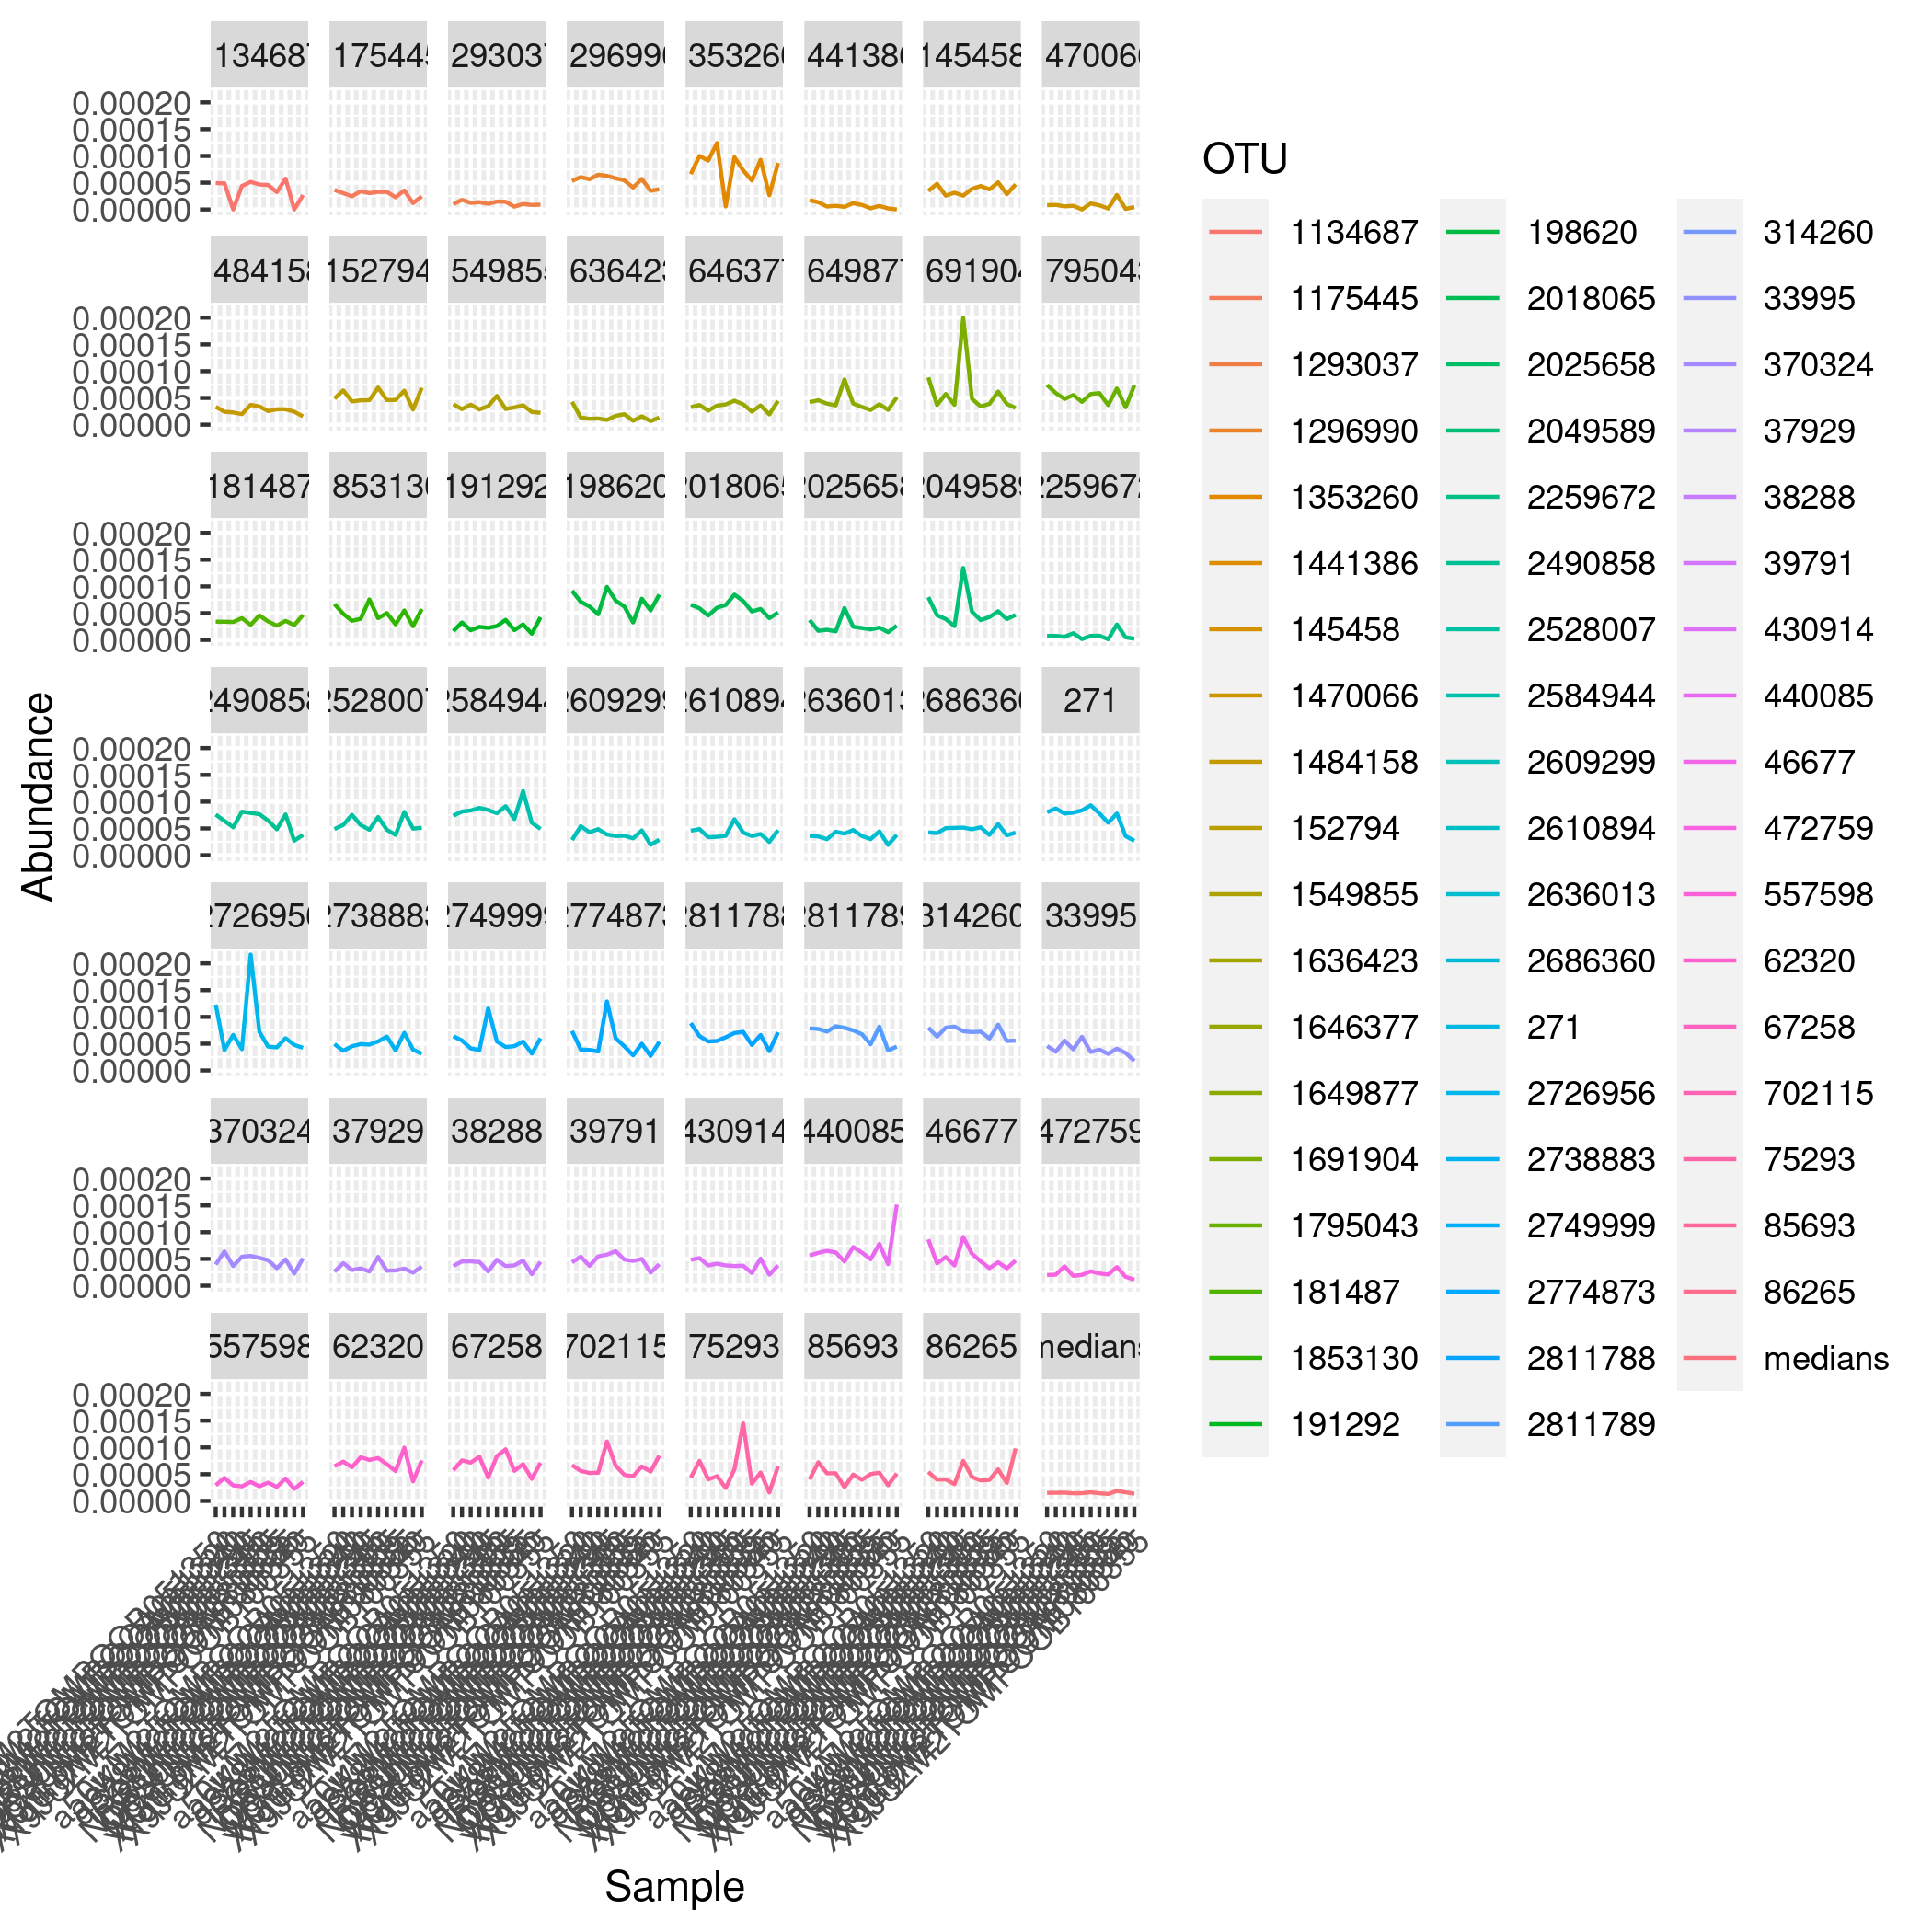
\includegraphics[scale = 0.8]{abundance_tomate_aleatorio1_9.csv_key_otus_medians.png}
   \caption{Plots representing relative abundance of each keystone OTU and one representing the median relative abundance  across samples of rhizosphere of tomate_aleatorio1_9.csv. Most keystone OTUs have relative abundance bigger than the median across all samples.  }
   \label{key_otus_vs_medians_tomate_aleatorio1_9.csv}
\end{figure}
\begin{figure}
 \centering
 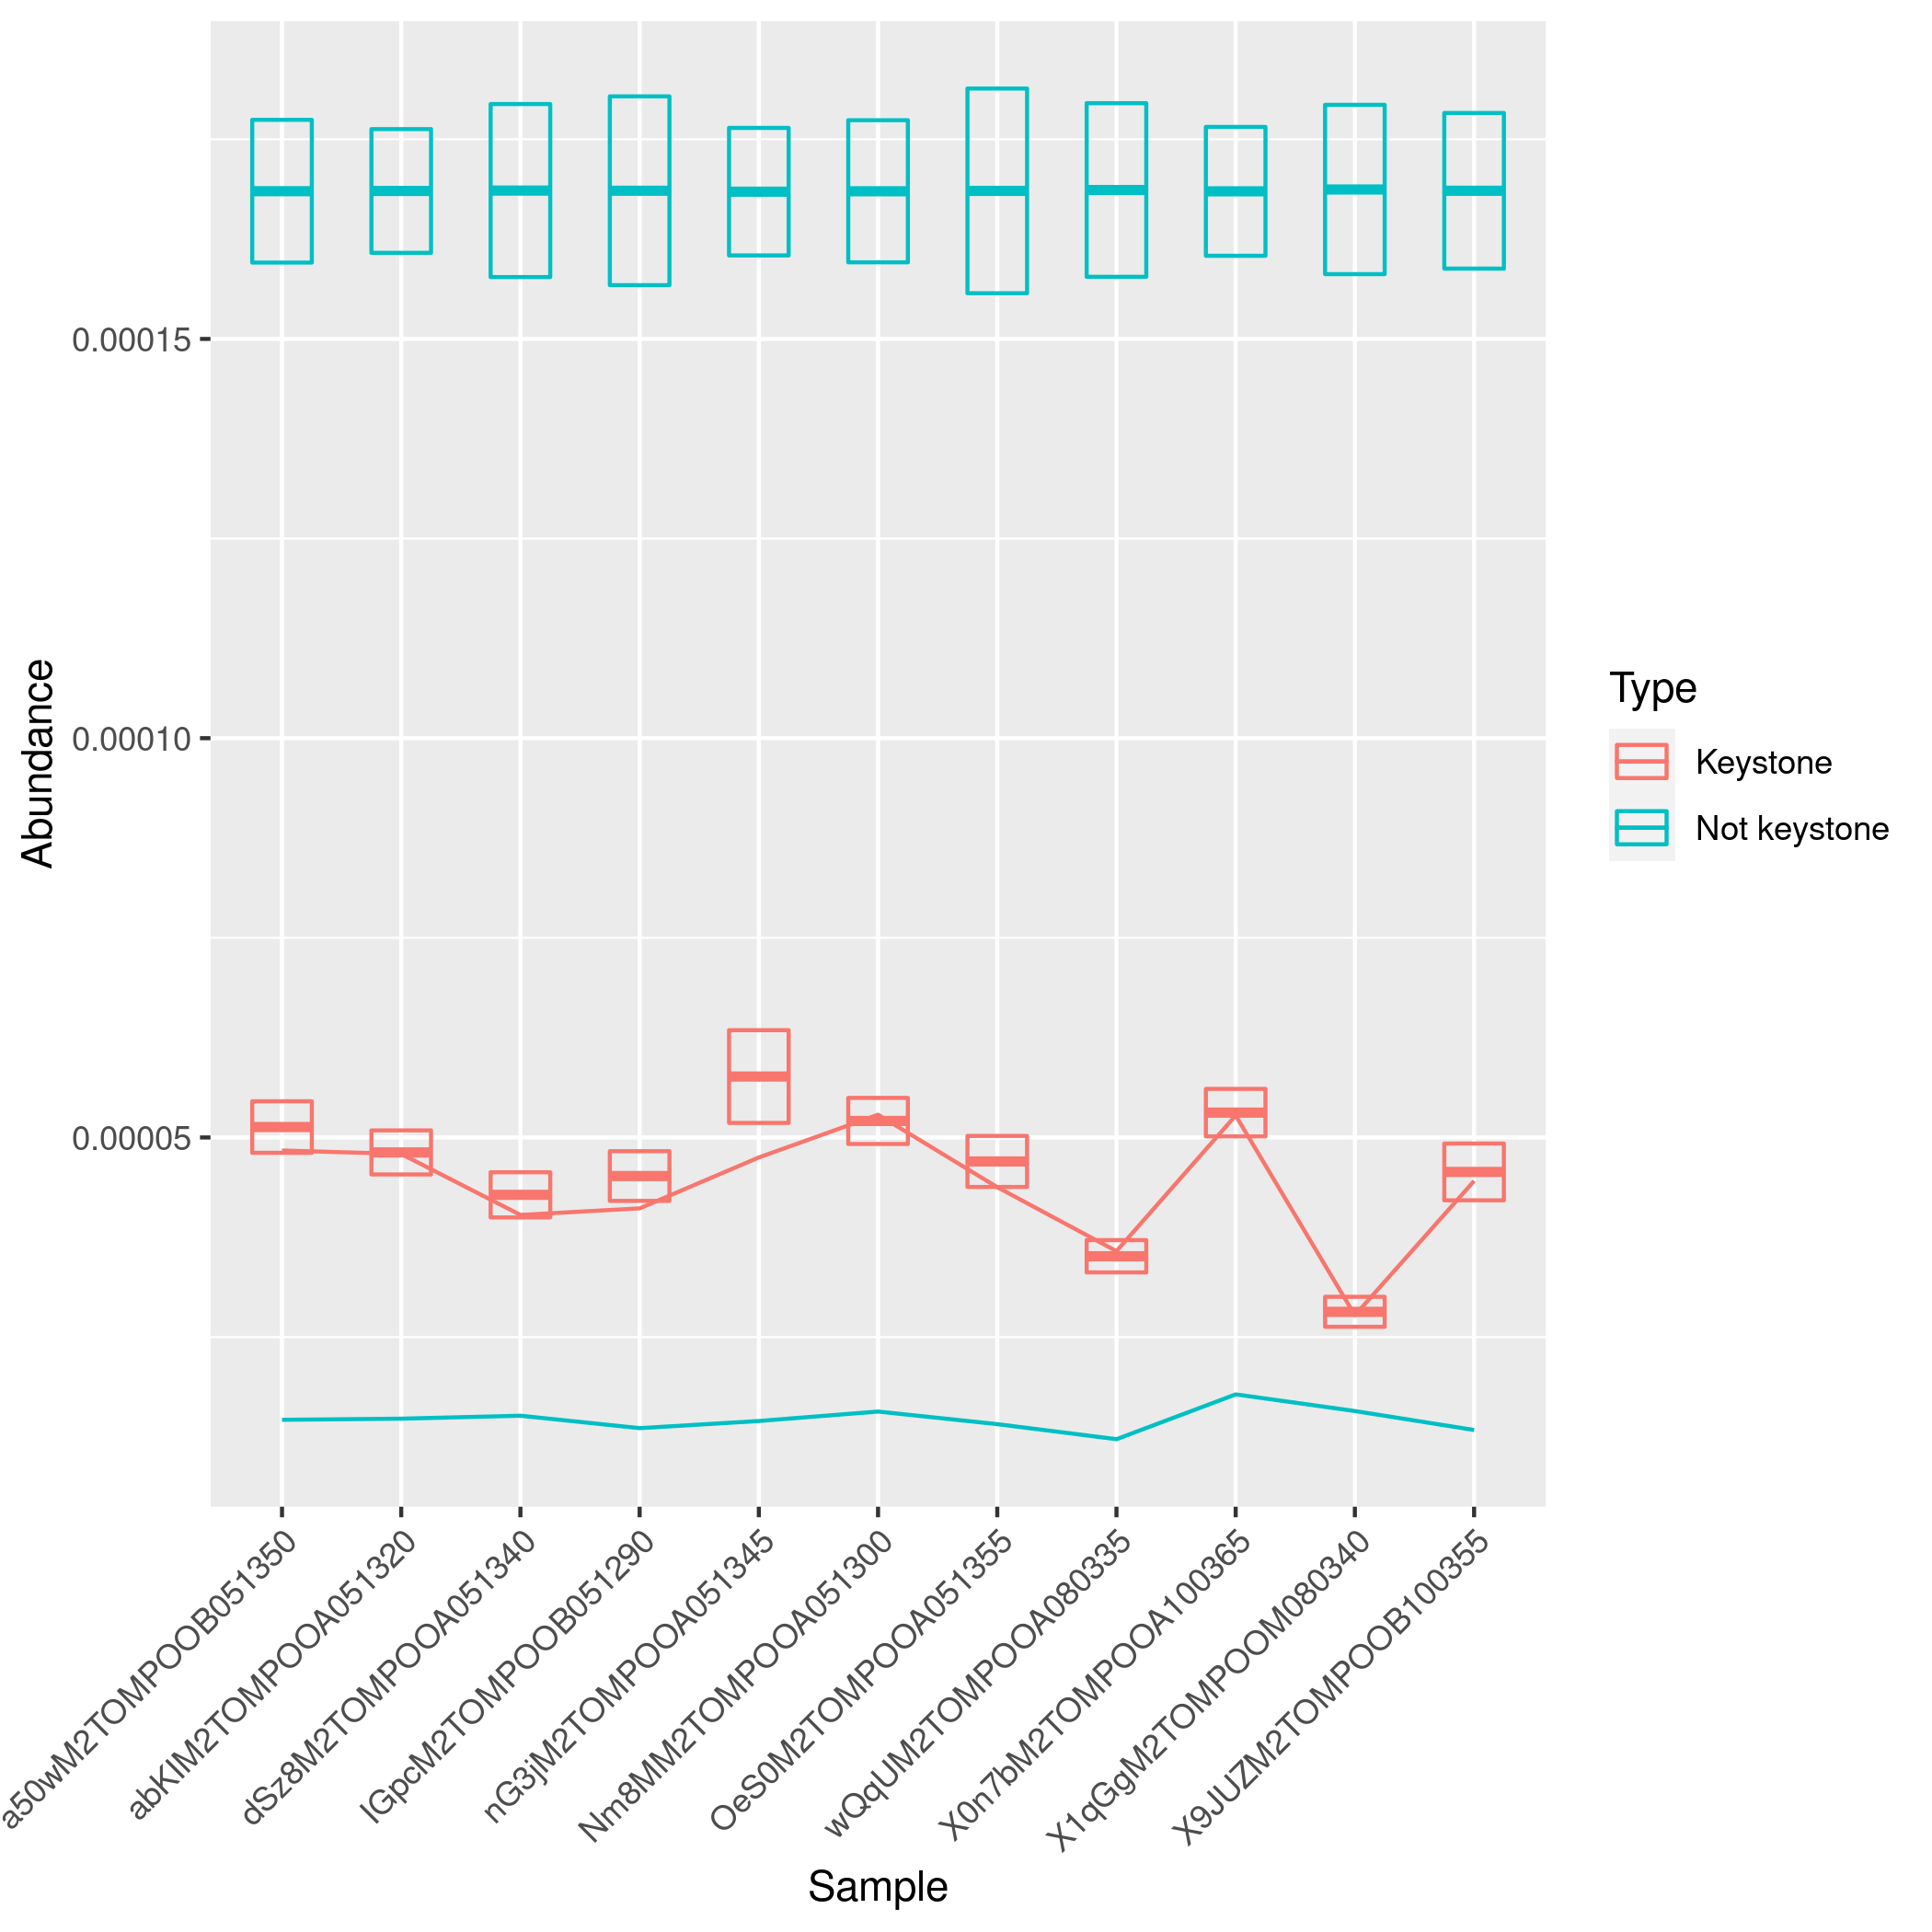
\includegraphics[scale = 0.75]{mean_median_key_vs_not_key_tomate_aleatorio1_9.csv.png}
\caption{Boxes represent mean and standard error in the distribution of corresponding samples. Lines represent the corresponding medians. In these samples of rhizosphere oftomate_aleatorio1_9.csv}
\label{mean_median_tomate_aleatorio1_9.csv}
\end{figure}
\begin{figure}
   \centering
   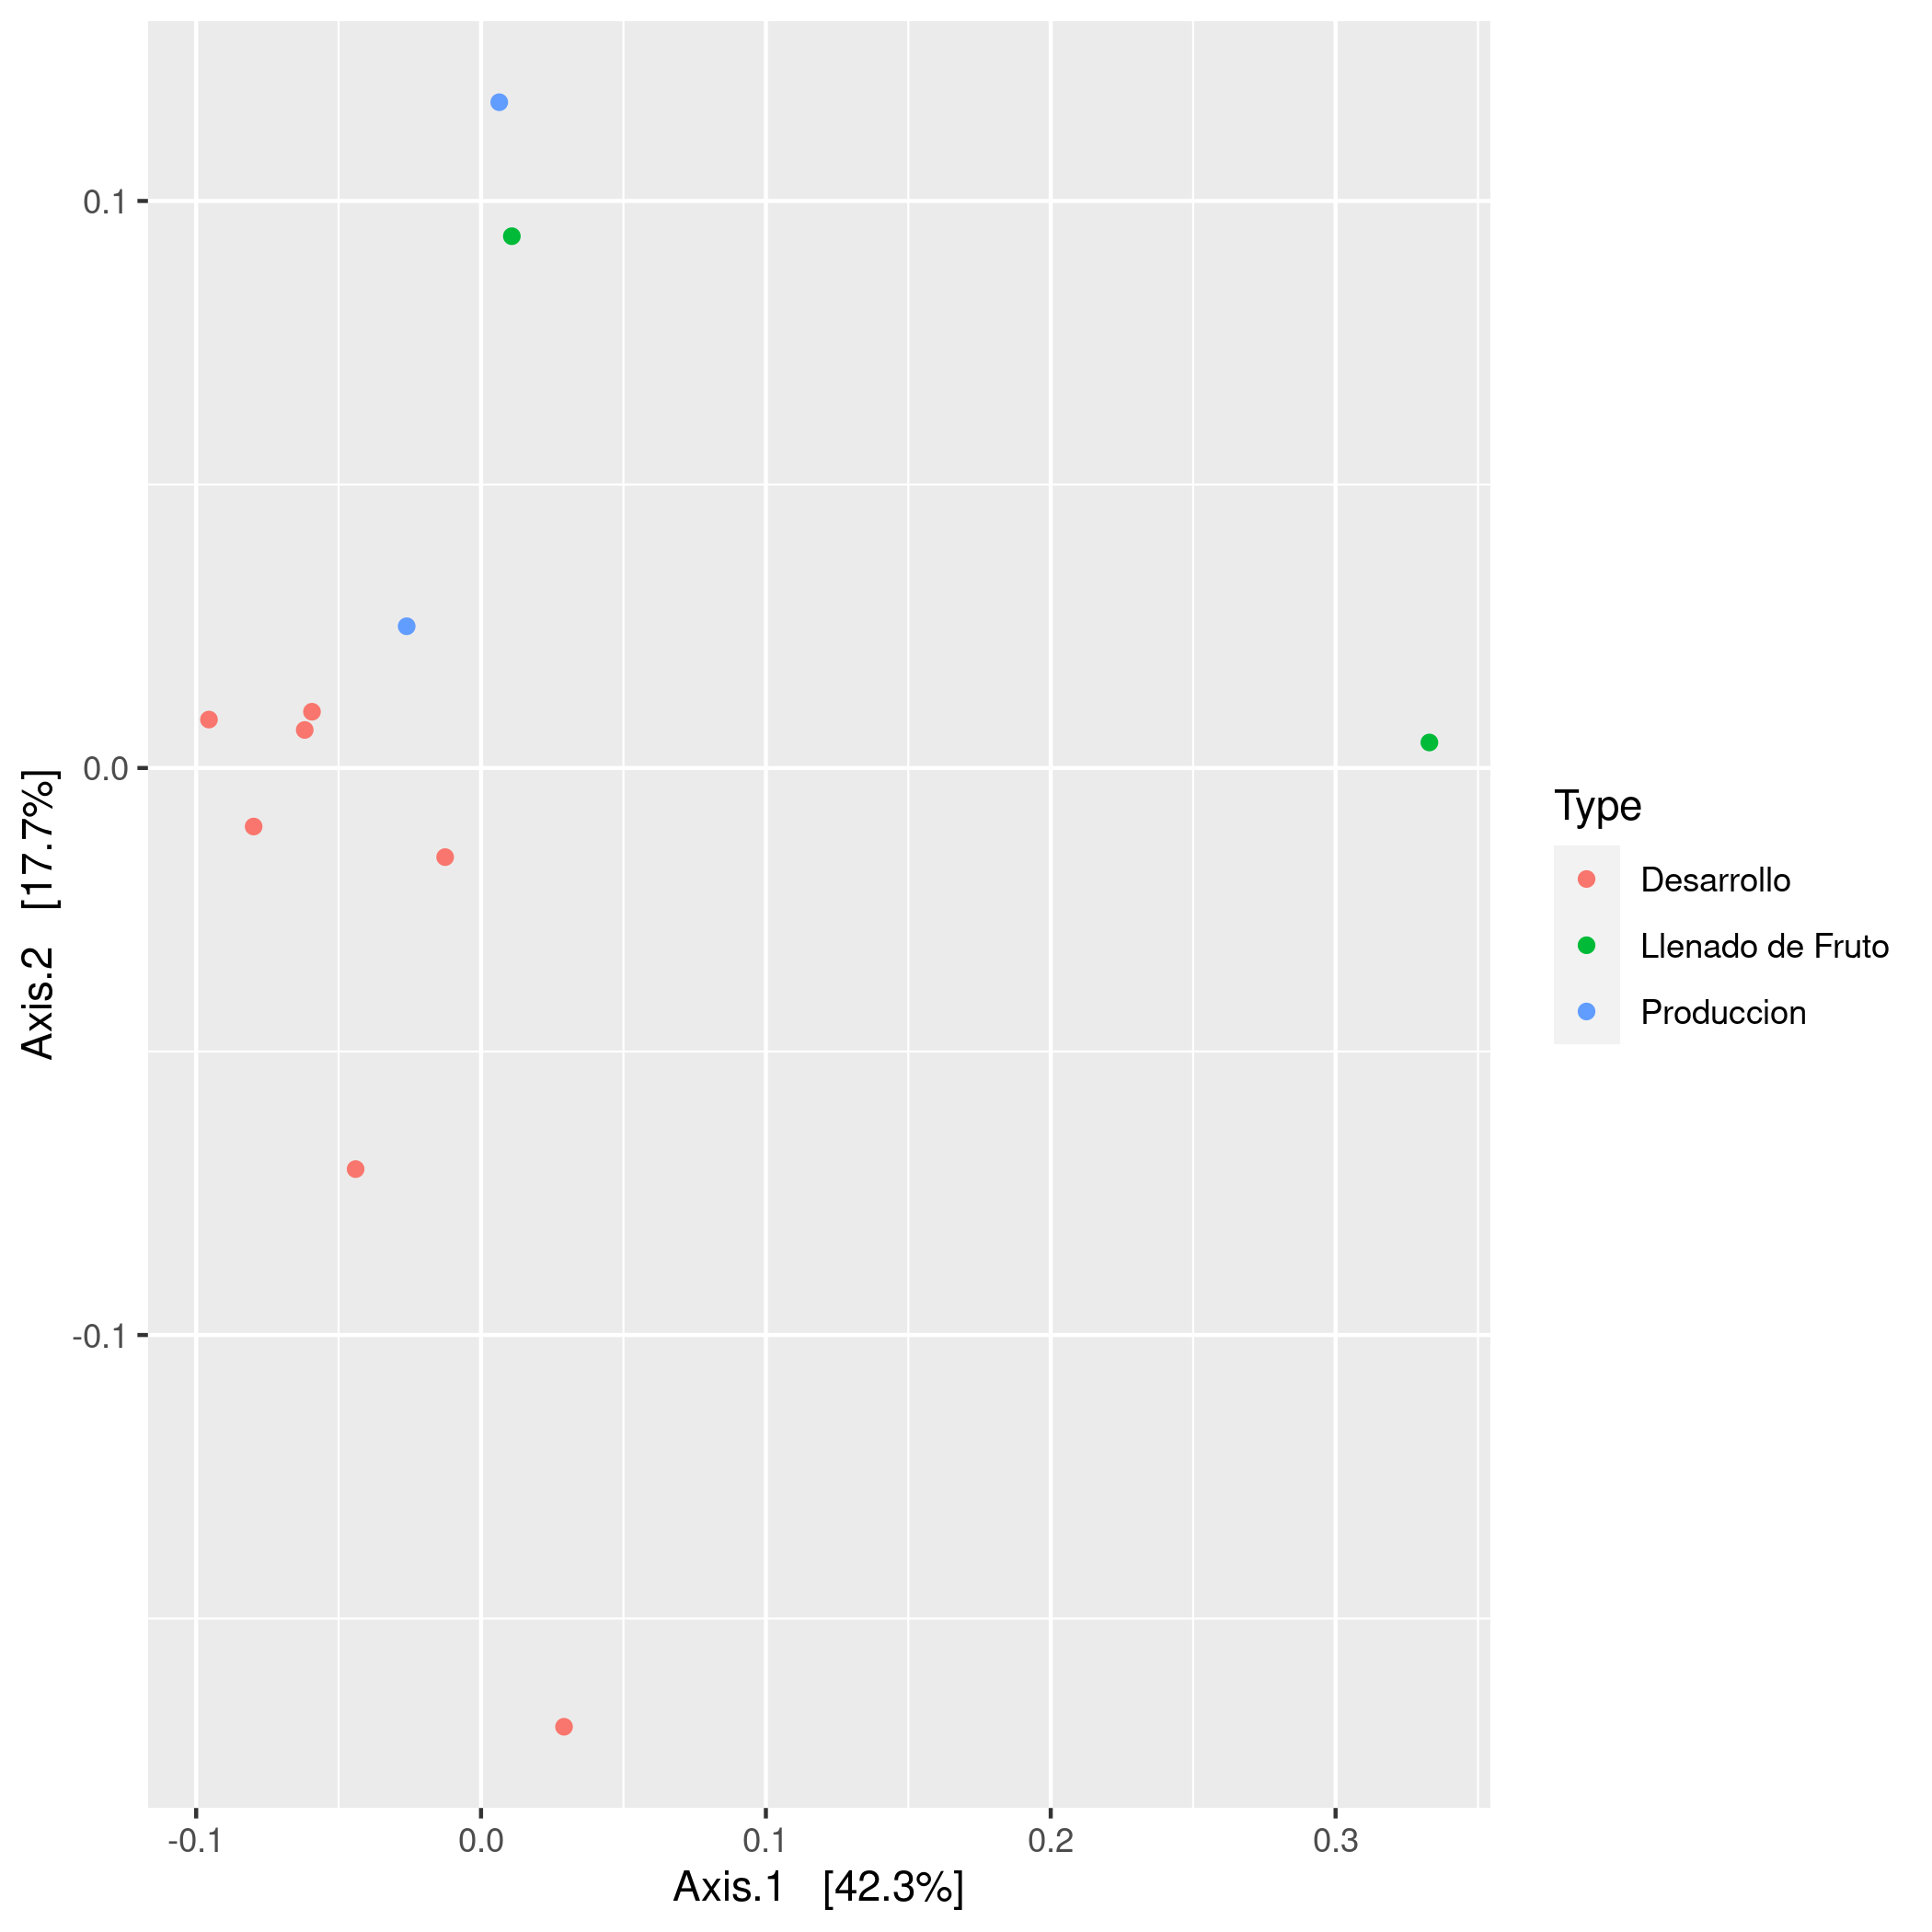
\includegraphics[scale = 0.7]{pcoa_muestras_tomate_aleatorio1_9.csv.png}
 \caption{PCoA analysis with Bray-Curtis distance of rhizosphere samples of tomate_aleatorio1_9.csv.}
 \label{fig:tomate_aleatorio1_9.csv_pcoa}
\end{figure}
\begin{figure}
  \centering
  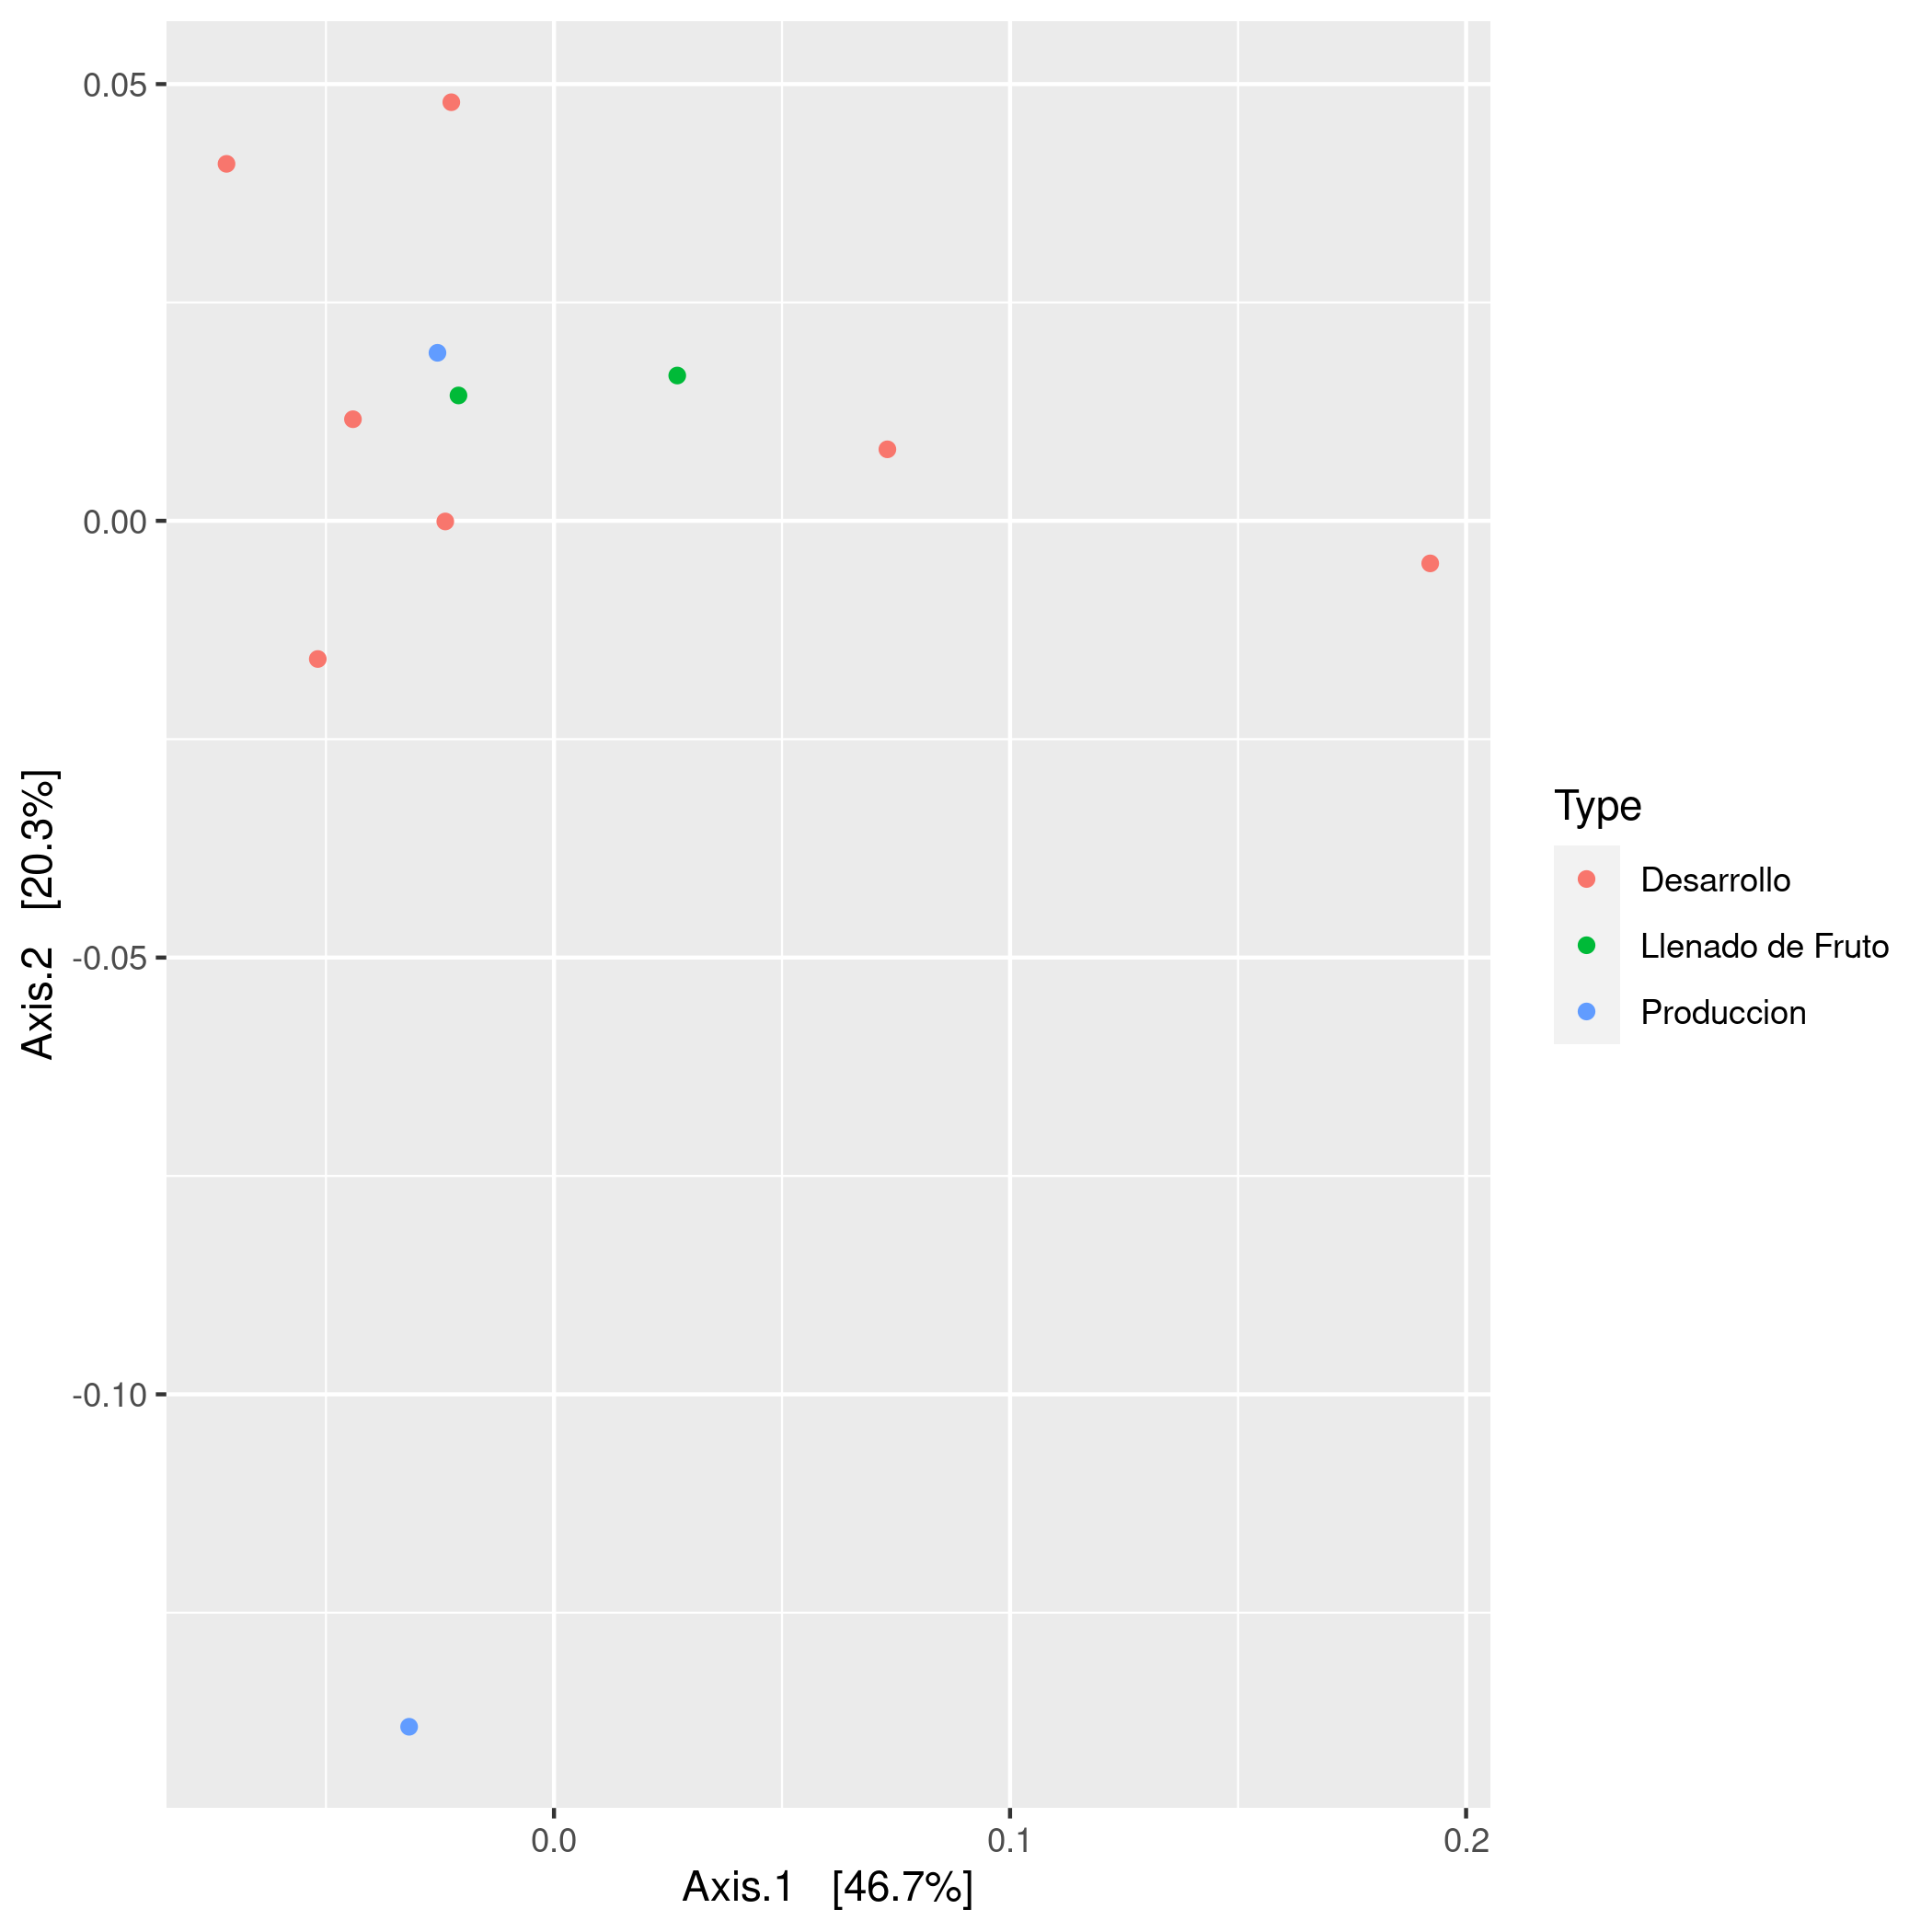
\includegraphics[scale = 0.7]{pcoa_key_otus_tomate_aleatorio1_9.csv.png}
  \caption{PCoA analysis with Bray-Curtis distance of rhizosphere samples of tomate_aleatorio1_9.csv, restricted to keystone OTUs.}
  \label{fig:tomate_aleatorio1_9.csv_pcoa_key_otus}
\end{figure}
